%# -*- coding: utf-8-unix -*-
%======================================================================
% my weekly-report.tex for recording my work!
%======================================================================
% 双面打印
\documentclass{qbook}
\addbibresource{bib/qbook.bib}  % 导入参考文献数据库

\usepackage{pdfpages}
%\includepdf[pages=-]{figure/pdf-1-gu-phd-thesis-extracted.pdf}

\usepackage{hyperref}
% \section{Hello World}
% \label{sec:hello}
% \hyperref[sec:hello]{Word of text}

\begin{document}
\pagestyle{empty}
%# -*- coding: utf-8-unix -*-
\thispagestyle{empty}
\begin{tikzpicture}[overlay,remember picture,font=\sffamily\bfseries]
\draw[ultra thick,c4,name path=big arc] ([xshift=-2mm]current page.north) arc(150:285:11)
coordinate[pos=0.225] (x0);
\begin{scope}
\clip ([xshift=-2mm]current page.north) arc(150:285:11) --(current page.north
east);
\fill[c4!50,opacity=0.25] ([xshift=4.55cm]x0) circle (4.55);
\fill[c4!50,opacity=0.25] ([xshift=3.4cm]x0) circle (3.4);
\fill[c4!50,opacity=0.25] ([xshift=2.25cm]x0) circle (2.25);
\draw[ultra thick,c4!50] (x0) arc(-90:30:6.5);
\draw[ultra thick,c4] (x0) arc(90:-30:8.75);
\draw[ultra thick,c4!50,name path=arc1] (x0) arc(90:-90:4.675);
\draw[ultra thick,c4!50] (x0) arc(90:-90:2.875);
\path[name intersections={of=big arc and arc1,by=x1}];
\draw[ultra thick,c4,name path=arc2] (x1) arc(135:-20:4.75);
\draw[ultra thick,c4!50] (x1) arc(135:-20:8.75);
\path[name intersections={of=big arc and arc2,by={aux,x2}}];
\draw[ultra thick,c4!50] (x2) arc(180:50:2.25);
\end{scope} 
\path[decoration={text along path,text color=c4,
	raise = -2.8ex,
	text  along path,
%	text = {|\sffamily\bfseries|\today},
	text = {|\sffamily\bfseries|2019},
	text align = center,
},
decorate
] ([xshift=-2mm]current page.north) arc(150:245:11);
%
\begin{scope}
\path[clip,postaction={fill=c3}]
([xshift=2cm,yshift=-8cm]current page.center) rectangle ++ (4.2,7.7);
\fill[c2] ([xshift=0.5cm,yshift=-8cm]current page.center)
([xshift=0.5cm,yshift=-8cm]current page.center)  arc(180:60:2)
|- ++ (-3,6) --cycle;
\draw[ultra thick,c4] ([xshift=-1.5cm,yshift=-8cm]current page.center) 
arc(180:0:2);
\draw[ultra thick,c4] ([xshift=0.5cm,yshift=-8cm]current page.center) 
arc(180:0:2);
\draw[ultra thick,c4] ([xshift=2.5cm,yshift=-8cm]current page.center) 
arc(180:0:2);
\draw[ultra thick,c4] ([xshift=4.5cm,yshift=-8cm]current page.center) 
arc(180:0:2);
\fill[red] ([xshift=2.5cm,yshift=-8cm]current page.center) +(60:2) circle(1.5mm);
\node[text=c5!80!black] at ([xshift=4.7cm,yshift=-5.2cm]current page.center) {$\rho:=\dfrac{1+\sqrt{-3}}{2}$};
\end{scope}
%
\fill[c1] ([xshift=2cm,yshift=-8cm]current page.center) rectangle ++ (-13.7,7.7);
\node[text=white,anchor=west,scale=4,inner sep=0pt] at
%([xshift=-10.55cm,yshift=-3cm]current page.center) {$\mathbb{ Q }$-book 书籍模板};
([xshift=-10.55cm,yshift=-3cm]current page.center) {马波book};
\node[text=white,anchor=west,scale=2,inner sep=0pt] at
([xshift=-4.5cm,yshift=-5.5cm]current page.center) {\quad 马波};
\end{tikzpicture}
  % 载入封面
\begin{center}
	\Large{\sffamily\bfseries\heiti Bo Ma} \\ \vspace{2em}
	\Large{\sffamily\bfseries\heiti 更新日期: \today} \\ \vspace{1em}
	\Large{\sffamily\bfseries\heiti 电话: \texttt{88231380}} \\
	\Large{\sffamily\bfseries\heiti 邮箱: \texttt{mabo@ihep.ac.cn}} \\
	
\end{center} 
\vfill
\vspace{30em}
\begin{tabular*}{\textwidth}{ccc}
	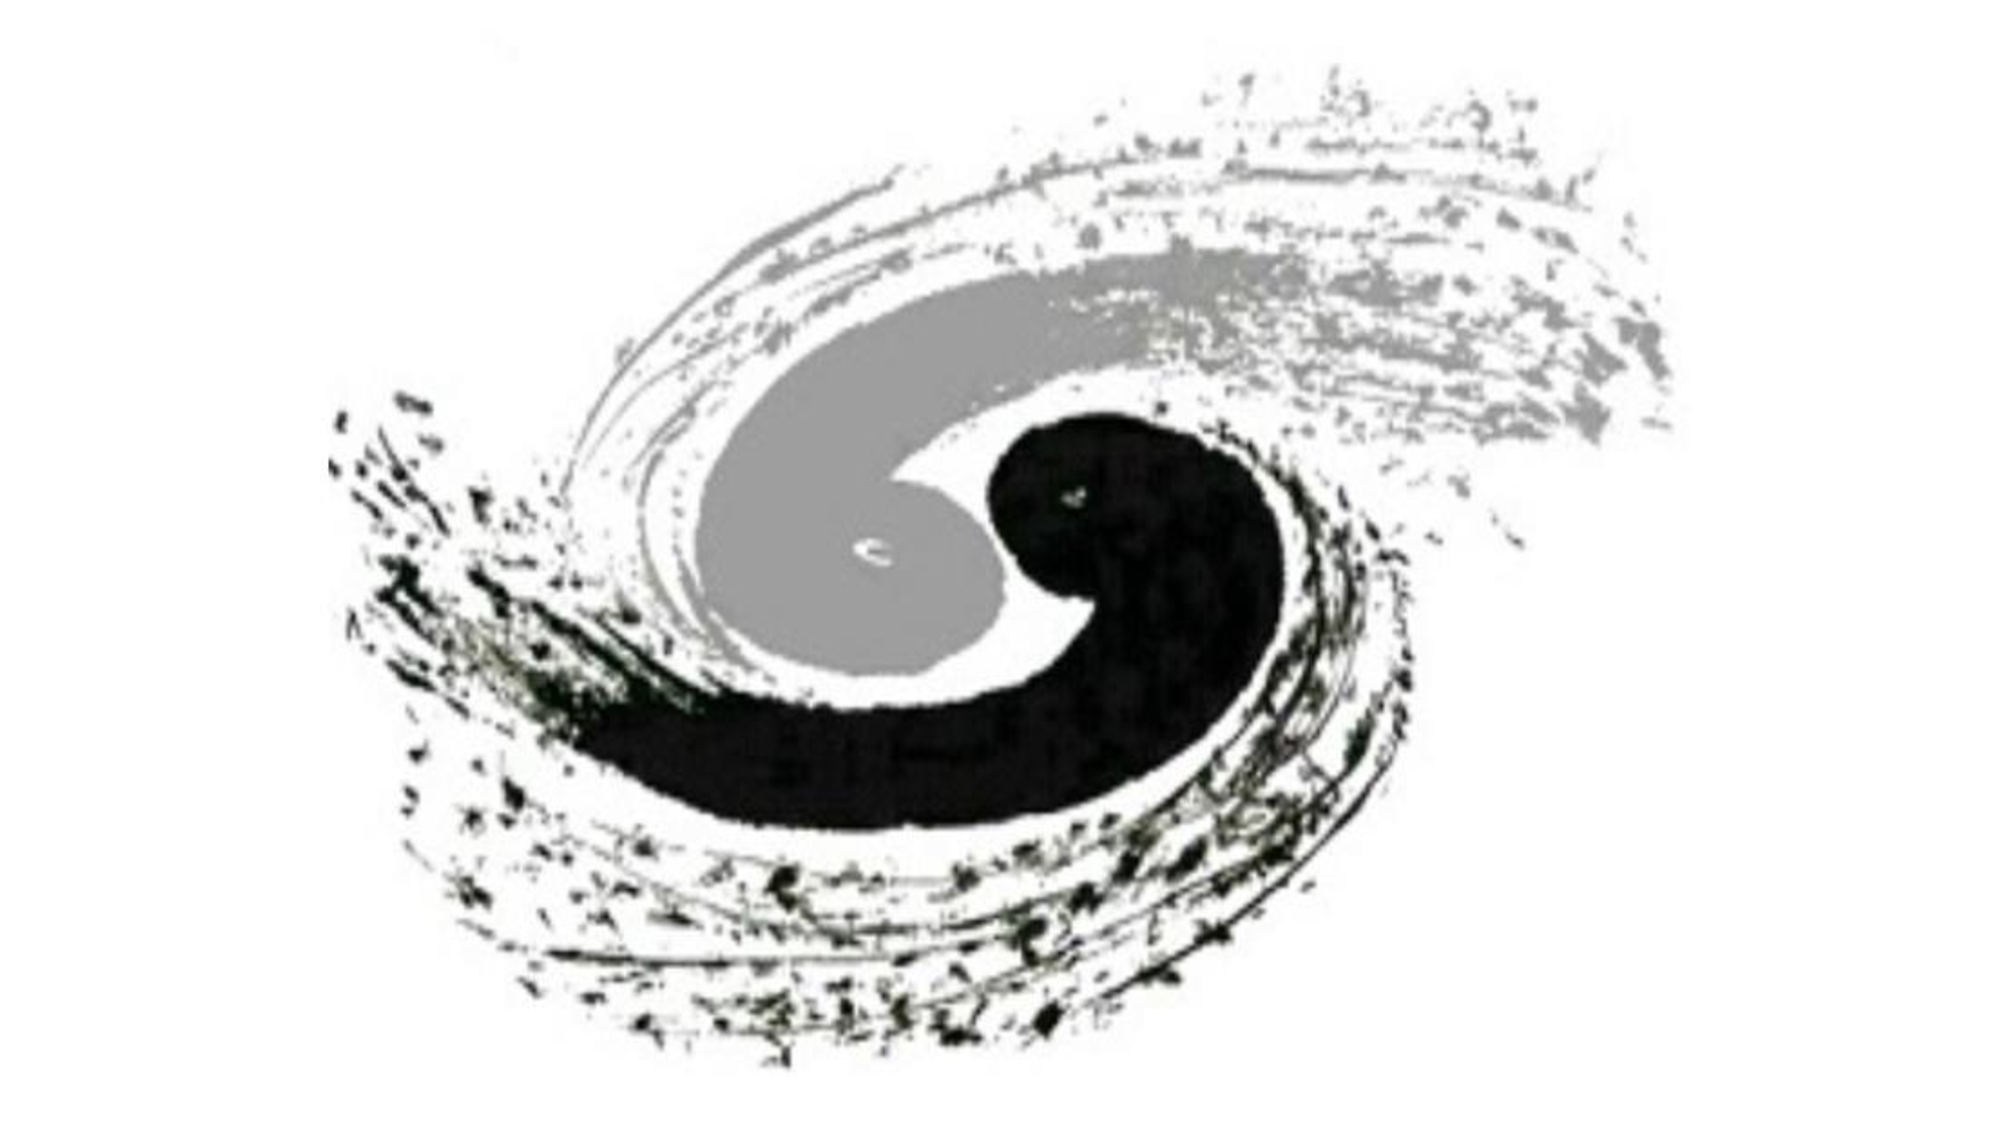
\includegraphics[width=0.3\textwidth]{figure/IHEP-LOGO.pdf}
	& \begin{minipage}[b]{0.6\textwidth}
		\small\sffamily
		中国科学院高能物理研究所\\
		 核技术应用研究中心\\
		北京市射线成像技术与装备工程技术研究中心\\
		Institute of High Energy Physics, 
		Chinese Academyof Sciences, Beijing 100049, China  
	\end{minipage}
\end{tabular*}  
\thispagestyle{empty}
\frontmatter  % 对前言和概览用罗马数字作为页码
\pagestyle{empty}

\begin{pre}
	\thispagestyle{empty}
	\begin{center}
		{\kaishu{吾日三醒吾身,吾周一结吾业}}
	\end{center}

\vspace*{5\baselineskip}
\centerline{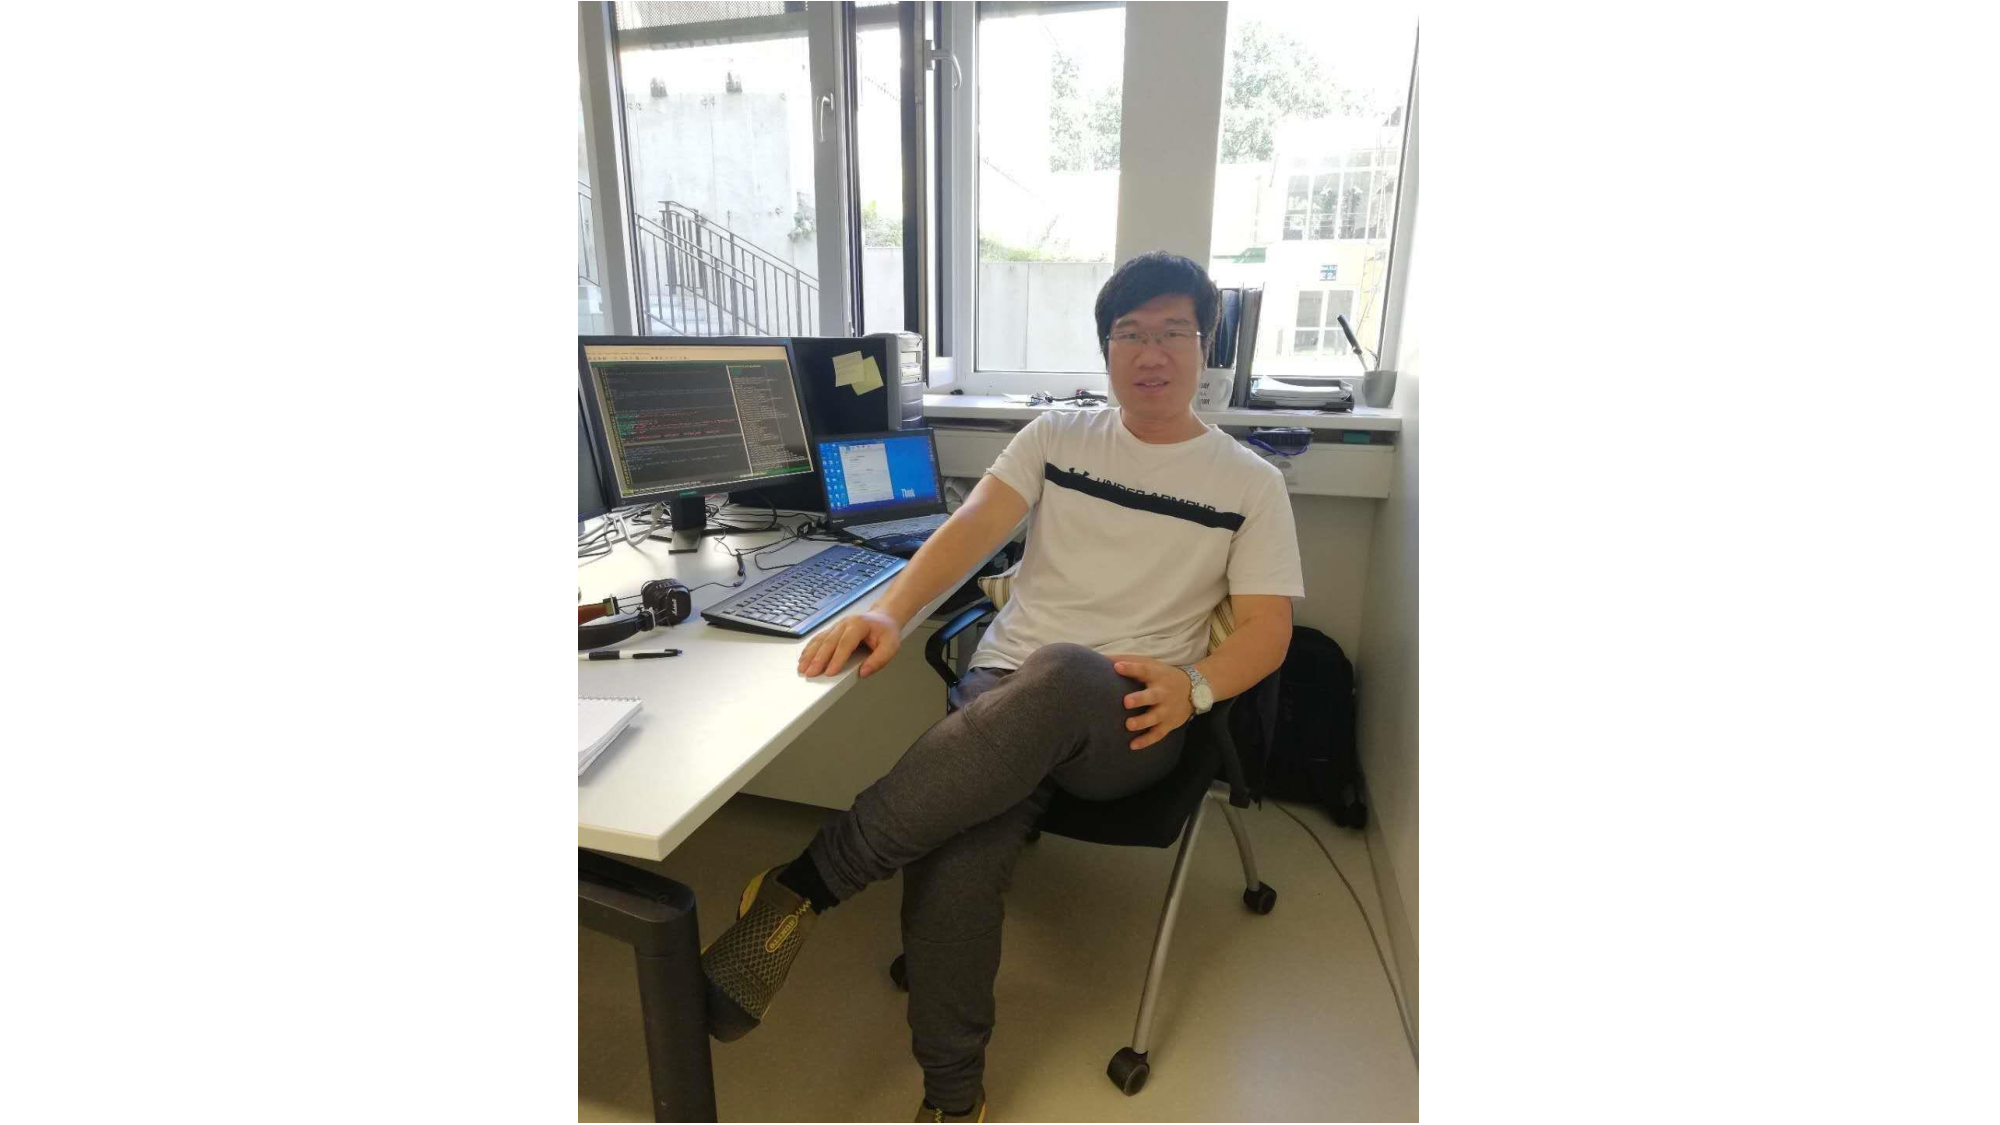
\includegraphics[scale=0.6]{figure/my-photo.pdf}}
\vspace*{1\baselineskip}
\centerline{\fontsize{26pt}{26pt}王霸之气}
\end{pre}
\pagestyle{empty}
\tableofcontents
\cleardoublepage
%# -*- coding: utf-8-unix -*-
\begin{overview}
\thispagestyle{empty}
朕自2019年5月回高能所工作,响应各层领导的号召,决定认真写好每一周的工作报告,认真总结一周的工作,同时做好下一周的工作计划,不但要低头干活,更要抬头看天,不浪费每一分钟的时间,争取获得更多的科研成果!Fighting!

\end{overview}
 
\mainmatter	  % 对正文用阿拉伯数字作为页码
%======================================================================
% 正文内容
\pagestyle{fancy}
\setcounter{page}{0}

% All personal defined new commands. 
% all the new commands I defined is here

%1: romman number.
%   #1: arabic number, like 1,2,3...

\newcommand{\myUpRoman}[1]{\uppercase\expandafter{\romannumeral#1}}

%2: color text, #1 : the color, such as red ,blue,etc.
%               #2: the text 

\newcommand{\myColorFonTxt}[2]{{\color{#1}#2}}
%note can not put the surffix of the file".tex"
% !TEX TS-program = xelatex
% !TEX encoding = UTF-8 Unicode
% !TEX root = ../qbook-latex-template.tex
% !TEX spellcheck = 
\chapter{Your content}

first chapter

\section{Your content-1}
%\includepdf[pages=-]{figure/pdf-1-gu-phd-thesis-extracted.pdf}

\subsection{Your content-1}
\subsection{Your content-1}
\subsection{Your content-1}



\backmatter	
%======================================================================
% 打印参考文献
\printbibliography[heading=bibintoc]
\makeatletter
\makeatother


\end{document}
